\documentclass[compress]{beamer}
\usepackage[
    title={Collaborative Learning},
    subtitle={Una soluzione di reinforcement learning applicata a un nodo router di messaggi},
    event={Progetto fine corso Machine Learning},
    author={DLP, MC, LF},
    longauthor={Daniele La Prova, Matteo Conti, Luca Falasca},
    email={},
    institute={ML 2023-2024},
    longinstitute={Universita' degli Studi di Roma Tor Vergata},
]{unislides}
\usepackage{graphicx} % Required for inserting images
\usepackage{minted}
\usepackage{algorithm}
\usepackage{hyperref}
\usepackage{adjustbox}

\begin{document}

\begin{frame}[plain]
    \titlepage
\end{frame}

\section*{Introduzione}
%TODO:

\subsection*{Contesto}
%TODO:

\subsection*{Obiettivi}
%TODO:

\section*{Metodologia}
%TODO:

\subsection*{Agente}
%TODO:

\subsubsection*{AgentFaçade}
%TODO:

\subsubsection*{AgentFactory}
%TODO:

\subsubsection*{Decisions}
%TODO:

\subsection*{Simulazione}
%TODO:

\subsubsection*{Nodo}
\begin{frame}{Nodo}
    E' l'elemento della rete che è in grado di ricevere e inviare messaggi sulla base della scelta dell'agente, è composto da:
    \begin{columns}
        \column{0.5\textwidth}
            \begin{minipage}[b]{1\textwidth}
                \begin{itemize}
                    \item Controller, che implementa la logica del nodo
                    \item AgentClient, che permette la comunicazione con l'agente
                    \item Queues, una o più code che accodano messaggi
                \end{itemize}
            \end{minipage}
        \column{0.5\textwidth}
            \begin{minipage}{1\textwidth}
                \begin{adjustbox}{margin=0cm 0cm 0.1cm 0.2cm, center} % left, bottom, right, top
                    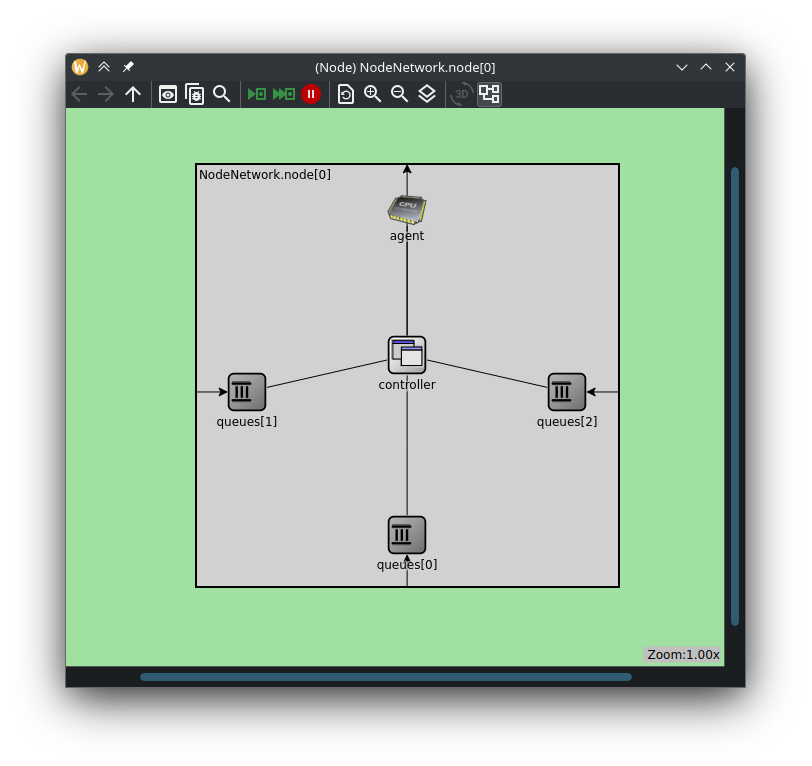
\includegraphics[width=1\textwidth]{figs/node_layout_3queues.png}
                \end{adjustbox}
            \end{minipage}
    \end{columns}
\end{frame}

\subsubsection*{Nodo - Controller}
\begin{frame}{Nodo - Controller (1)}
E' il componente che implementa la logica del nodo, in particolare:
\vspace{0.5cm}
    \begin{columns}
        \column{0.6\textwidth}
            \begin{minipage}[b]{1\textwidth}
                \begin{itemize}
                    \item Campiona lo stato visibile al nodo
                    \item Interroga l'agente per ottenere l'azione consegnandogli la reward dell'azione precedente
                    \item Attua l'azione ricevuta dall'agente
                    \item Calcola la reward per le azioni ricevute dall'agente
                \end{itemize}
            \end{minipage}
        \column{0.4\textwidth}
            \begin{minipage}{.9\textwidth}
                \begin{adjustbox}{margin=0.5cm 0cm 0.1cm 0.2cm, center} % left, bottom, right, top
                    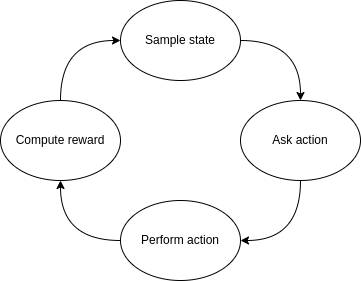
\includegraphics[width=1\textwidth]{figs/control_loop.png}
                \end{adjustbox}
            \end{minipage}
    \end{columns}
\end{frame}

\begin{frame}{Nodo - Controller (2)}
    Il controller si occupa anche di gestire le sorgenti energetiche del nodo, in particolare:
    \vspace{0.5cm}
        \begin{columns}
            \column{0.6\textwidth}
                \begin{minipage}[b]{1\textwidth}
                    \begin{itemize}
                        \item Una batteria, la cui carica dipende da fattori ambientali
                        \item Una presa di corrente, che ha un costo di utilizzo
                    \end{itemize}
                \end{minipage}
            \column{0.4\textwidth}
                \begin{minipage}{.9\textwidth}
                    \begin{adjustbox}{margin=0.5cm 0cm 0.1cm 0.2cm, center} % left, bottom, right, top
                        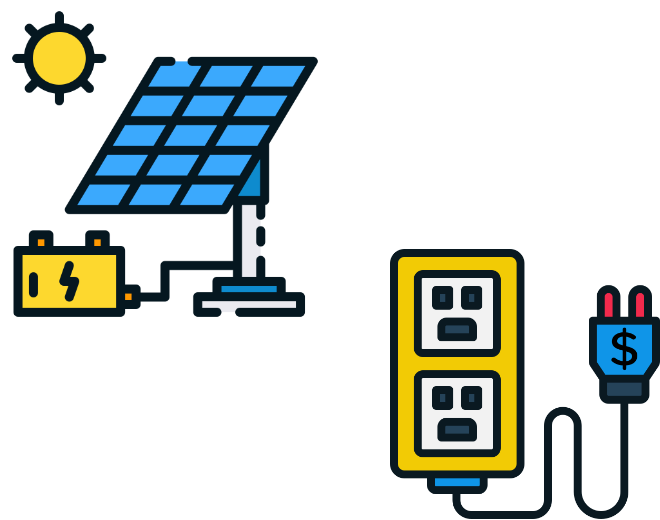
\includegraphics[width=1\textwidth]{figs/socket_battery.png}
                    \end{adjustbox}
                \end{minipage}
        \end{columns}
    \end{frame}

\subsubsection*{Nodo - Agent Client}
\begin{frame}{Nodo - Agent Client}
    E' il componente che fa da intermediario tra il controller e l'agente, in particolare:
    \begin{itemize}
        \item Accoglie le action request del controller, le quali contengono stato e reward dell'azione precedente 
        \item Converte l'action request in una bean compatibile con l'implementazione Python dell'agente
        \item Inoltra la bean all'agente
        \item Accoglie le bean di risposta dell'agente, le quali contengono l'azione da attuare
        \item Converte la bena di risposta in una action response compatibile con l'implementazione in C++ del controller
        \item Inoltra l'action response al controller
    \end{itemize}
\end{frame}

\subsubsection*{Nodo - Queue}
\begin{frame}{Nodo - Queue}
    E' il componente che implementa la logica della coda, in particolare:
    \vspace{0.5cm}
        \begin{columns}
            \column{0.6\textwidth}
                \begin{minipage}[b]{1\textwidth}
                    \begin{itemize}
                        \item Accoglie i pacchetti in arrivo, scartandoli se la coda è piena
                        \item Riceve le QueueDataRequest di pacchetti da parte del controller
                        \item Consegna i pacchetti al controller in delle QueueDataResponse
                        \item Comunica al controller gli aggiornamenti sullo stato della coda, tramite una QueueStateUpdate, ogni volta che arriva un pacchetto
                    \end{itemize}
                \end{minipage}
            \column{0.4\textwidth}
                \begin{minipage}{.9\textwidth}
                    \begin{adjustbox}{margin=0.5cm 0cm 0.1cm 0cm, center} % left, bottom, right, top
                        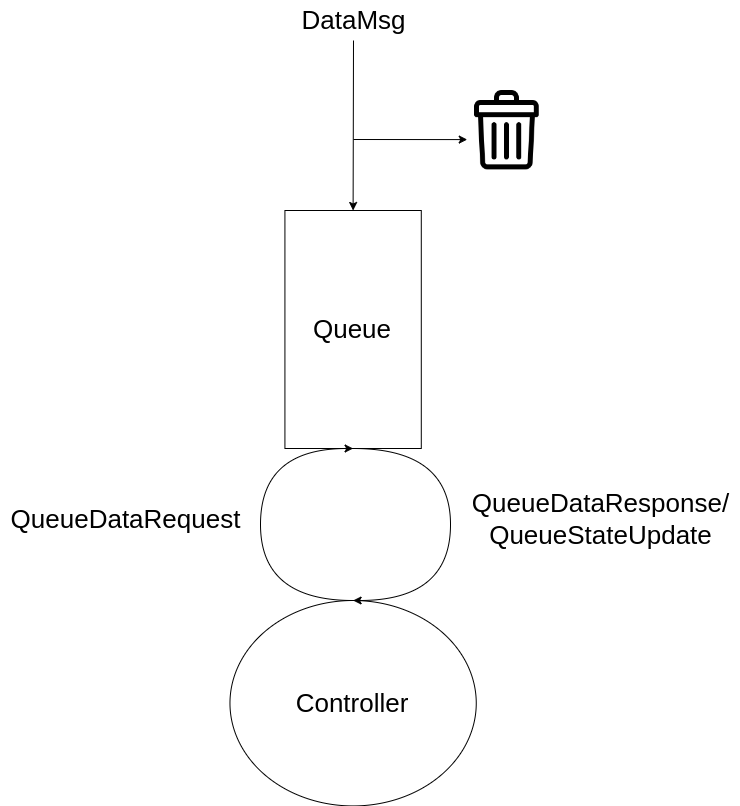
\includegraphics[width=1\textwidth]{figs/queue_scheme.png}
                    \end{adjustbox}
                \end{minipage}
        \end{columns}
\end{frame}

\subsubsection*{SrcNode}
\begin{frame}{SrcNode}
    E' l'elemento della rete che si occupa di generare il traffico, ogni Queue ha associato un SrcNode.
    Il tempo di interarrivo dei pacchetti è regolato da una distribuzione esponenziale con tasso $\lambda$ configurabile, mentre la dimensione dei pacchetti è regolata da una distribuzione uniforme su un intervallo configurabile.
    \begin{adjustbox}{margin=0.5cm 0cm 0.5cm 0.5cm, center} % left, bottom, right, top
        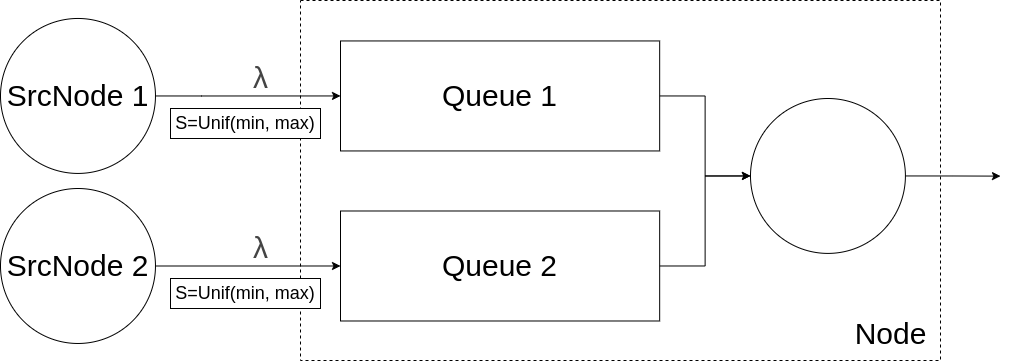
\includegraphics[width=.8\textwidth]{figs/src_scheme.png}
    \end{adjustbox}
\end{frame}

\subsubsection*{Network}
\begin{frame}{Network}
E' l'ambiente in cui vivono tutti gli elementi della simulazione, qui vengono specificati i collegamenti tra i SrcNode e le code del nodo router. 
    \begin{adjustbox}{margin=0cm 0cm 0cm 0cm, center} % left, bottom, right, top
        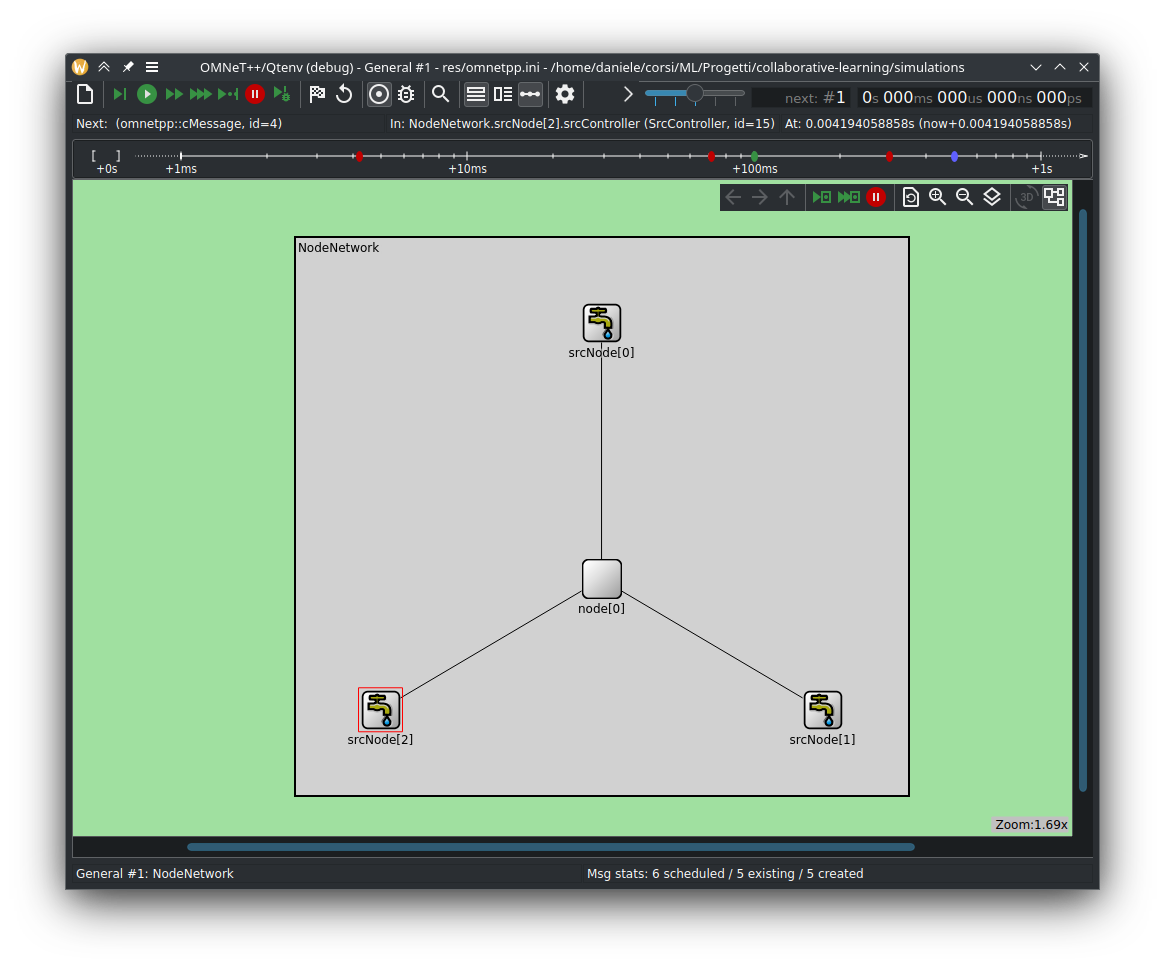
\includegraphics[width=.65\textwidth]{figs/network_layout_3queues.png}
    \end{adjustbox}
\end{frame}


\section*{Risultati}
%TODO:

\subsection*{Condizioni}

% TODO: una subsection per ogni scenario

\section*{Conclusioni}
%TODO:

\subsection*{What we have learned?}
%TODO:

\subsection*{What we could improve?}
%TODO:

\end{document}
